\documentclass[draft]{beamer}
%\documentclass{beamer}

\usepackage{graphicx}
\title[Prime Numbers]{Prime Numbers and the Riemann Hypothesis}
\subtitle{(Writing a book with Barry Mazur)}
\author[W.\thinspace{}Stein]{William Stein}
\date[Mazur 80]{June 4, 2018 at Harvard University}
\institute[SageMath, Inc. \& UW]{SageMath, Inc. and University of Washington}

\begin{document}

\begin{frame}
  \titlepage
\end{frame}

\begin{frame}{Abstract}
  \begin{abstract}
    In 2004, Barry Mazur and I started writing the
    book ``Prime Numbers and the Riemann Hypothesis'', which we recently
    published with Cambridge University Press. I'll talk about
    what's in the book and why, describe some of the technical aspects
    of production of the book, and tradeoffs for us between
    self publishing online versus with a traditional publisher.

    \vspace{.3in}
    This is talk about talking about the Riemann Hypothesis.
  \end{abstract}
\end{frame}

\begin{frame}{Overview}
  \tableofcontents
\end{frame}

\begin{frame}{Here's the book...}
  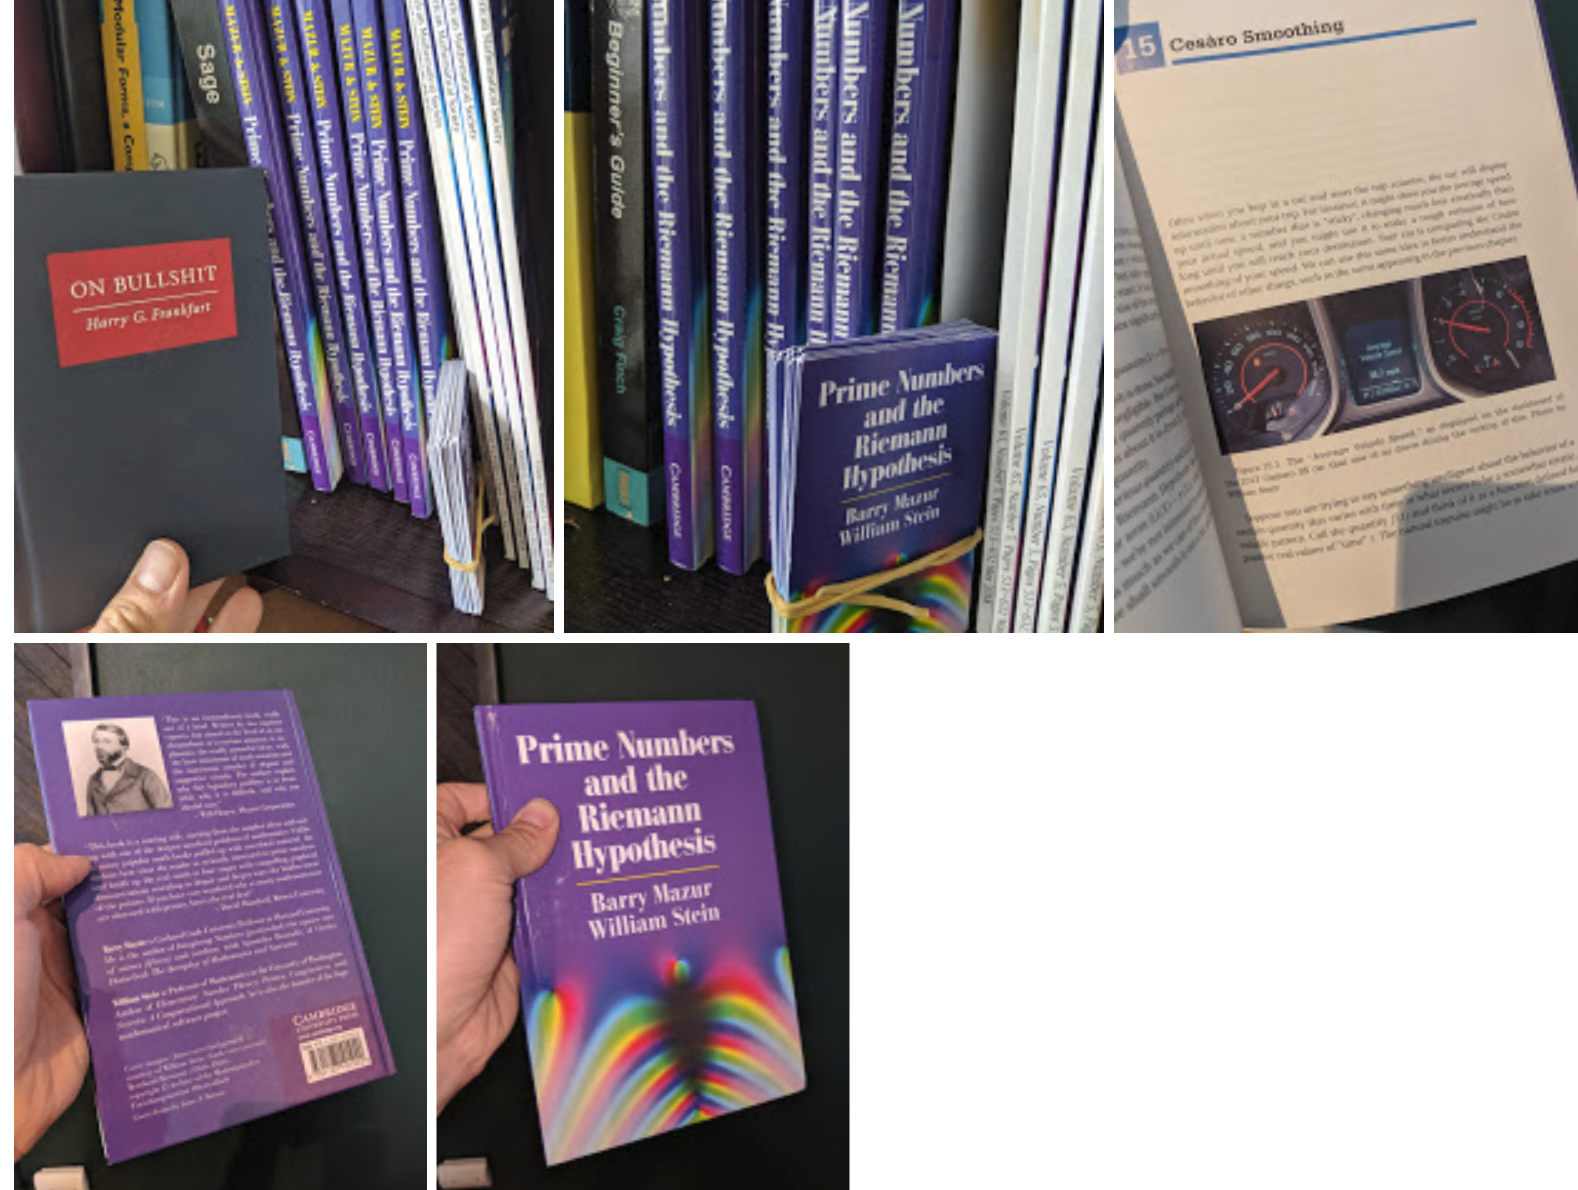
\includegraphics[width=.98\textwidth]{pics/the-book.png}
\end{frame}

\section{2005: CMI Public Lecture}

\begin{frame}{Clay Math Institute public lecture (MIT, May 3, 2005)}

  \href{http://www.claymath.org/library/public\_lectures/mazur\_riemann\_hypothesis.pdf}{\bf Are there still unsolved problems about the numbers 1, 2, 3, 4, ... ?}
  \vfill

  \begin{itemize}
    \item  Talk for a really general public audience (high school...)
    \item  Choose a problem to ``sell'' number theory to the general public:
          \begin{itemize}
            \item   Immediately accessible
            \item   Immediately interesting
            \item   Primes and how eratic they are
            \item   Cicada's every 13, 17 years...
            \item   Lots of examples that are "opening, interesting questions/issues."
            \item   People can immediately make computations of their \underline{own}
            \item   Barry Mazur got his father who had done NO
                  math hooked on Goldbach Conjecture, so thought
                  primes would work.
          \end{itemize}
  \end{itemize}
\end{frame}

\begin{frame}{SageMath}
  \vfill
  \begin{center}
    
\includegraphics[width=.5\textwidth]{pics/sage-logo.png}
  \end{center}
  \vfill

  I launched Sage a few months before this CMI public lecture.
  \begin{itemize}
    \item Sage is a free open source alternative to Mathematica, Maple, Magma, and Matlab.
    \item Early Sage development was motivated by this talk
          \begin{itemize}
            \item Linking Sage to Mathematica to compute the incomplete Gamma function.
            \item Early plotting functionality.
          \end{itemize}
  \end{itemize}
\end{frame}

\begin{frame}{The Prime Counting Problem}
  Let $\pi(x)$ be the number of primes $\leq x$.
  Problem: give a ``good approximation'' for $\pi(x)$

\end{frame}

\section{2006: Let's write a book!}

\begin{frame}{What kind of book?}
  \begin{itemize}
    \item   Book motivated by the prime counting problem (connect with other project -- explicit formula projects...).
    \item Mostly math and no "stories of people", since many other books do that already.
    \item  Similar to guessing rank of MW of elliptic curve from $a_p$.
    \item Bullshit
    \item T.\thinspace{}C. MITS
  \end{itemize}

\end{frame}

\begin{frame}{Our Approach}
  \begin{itemize}
    \item Do not emphasize people/history/stories, since that's done already in many other books.
    \item   Go back 150+ years and explain what RH is more from the point of view of real Fourier analysis and distributions.
          \begin{itemize}
            \item make big deal of the fact that we take mid-19th century real perspective
            \item leaving complex number to the very, very end.
          \end{itemize}
  \end{itemize}
\end{frame}

\begin{frame}{SageMath again}
  Used Sage to compute with prime numbers, zeros, etc., and generally to plot everything in the book.
  \begin{itemize}
    \item drawing tons of plots
    \item started book at same time as sage...
    \item plots absolutely essential to exposition
    \item surprising that you see the spikes with such little computation.
    \item take fourier transform of discrete distribution at primes, you get discrete distribution of zeros
    \item do the reverse get the discrete distribution of prime powers.
    \item without much power... that is striking:
    \item that is what got us thinking about "how explicit is the explicit formula if you compute".
  \end{itemize}
\end{frame}

\begin{frame}{SIMUW 2007: Test on High School Students}

  \url{https://wstein.org/edu/2007/simuw07/}
\end{frame}


\section{2013: Let's keep writing a book!}


\begin{frame}{Collaborative LaTeX via CoCalc}
  \begin{itemize}
    \item Using CoCalc's latex editor.
          \begin{itemize}
            \item web browser...
            \item gives a sense of the collaborative spirit
          \end{itemize}
    \item We put our PDF on the web at every stage.
    \item GitHub versions: \url{https://github.com/williamstein/rh}
  \end{itemize}
\end{frame}


\section{2014: Let's publish}

\begin{frame}{How to Publish the book:  Self publish!?}
  \begin{itemize}
    \item Self publishing: just put it on my website and see what happens.
          \begin{itemize}
            \item Enormous number of people that proof read it.
            \item Will Hearst pushed us for proper publication.
          \end{itemize}
  \end{itemize}
\end{frame}

\begin{frame}{Finding a commercial publisher}
  \begin{itemize}
    \item   Finding a publisher
    \item what expected to give is latex, and expect.
  \end{itemize}
\end{frame}


\begin{frame}{Typos and Mistakes}
  \begin{itemize}
    \item Dozens of people "on the internet" carefully read drafts of
          the book and provided incredibly useful feedback.  \textbf{THANKS!}
    \item The publisher also had a copy editor read the book,
          and provided very different feedback.
    \item Advice: never expect your publisher to catch the sort of
          mistakes somebody who cares about mathematics catches.
  \end{itemize}
\end{frame}


\begin{frame}{Production}

  \begin{itemize}
    \item cambridge might have made some positive steps toward latex
    \item net very positive overall experience.
  \end{itemize}

\end{frame}

\begin{frame}{Published!}

  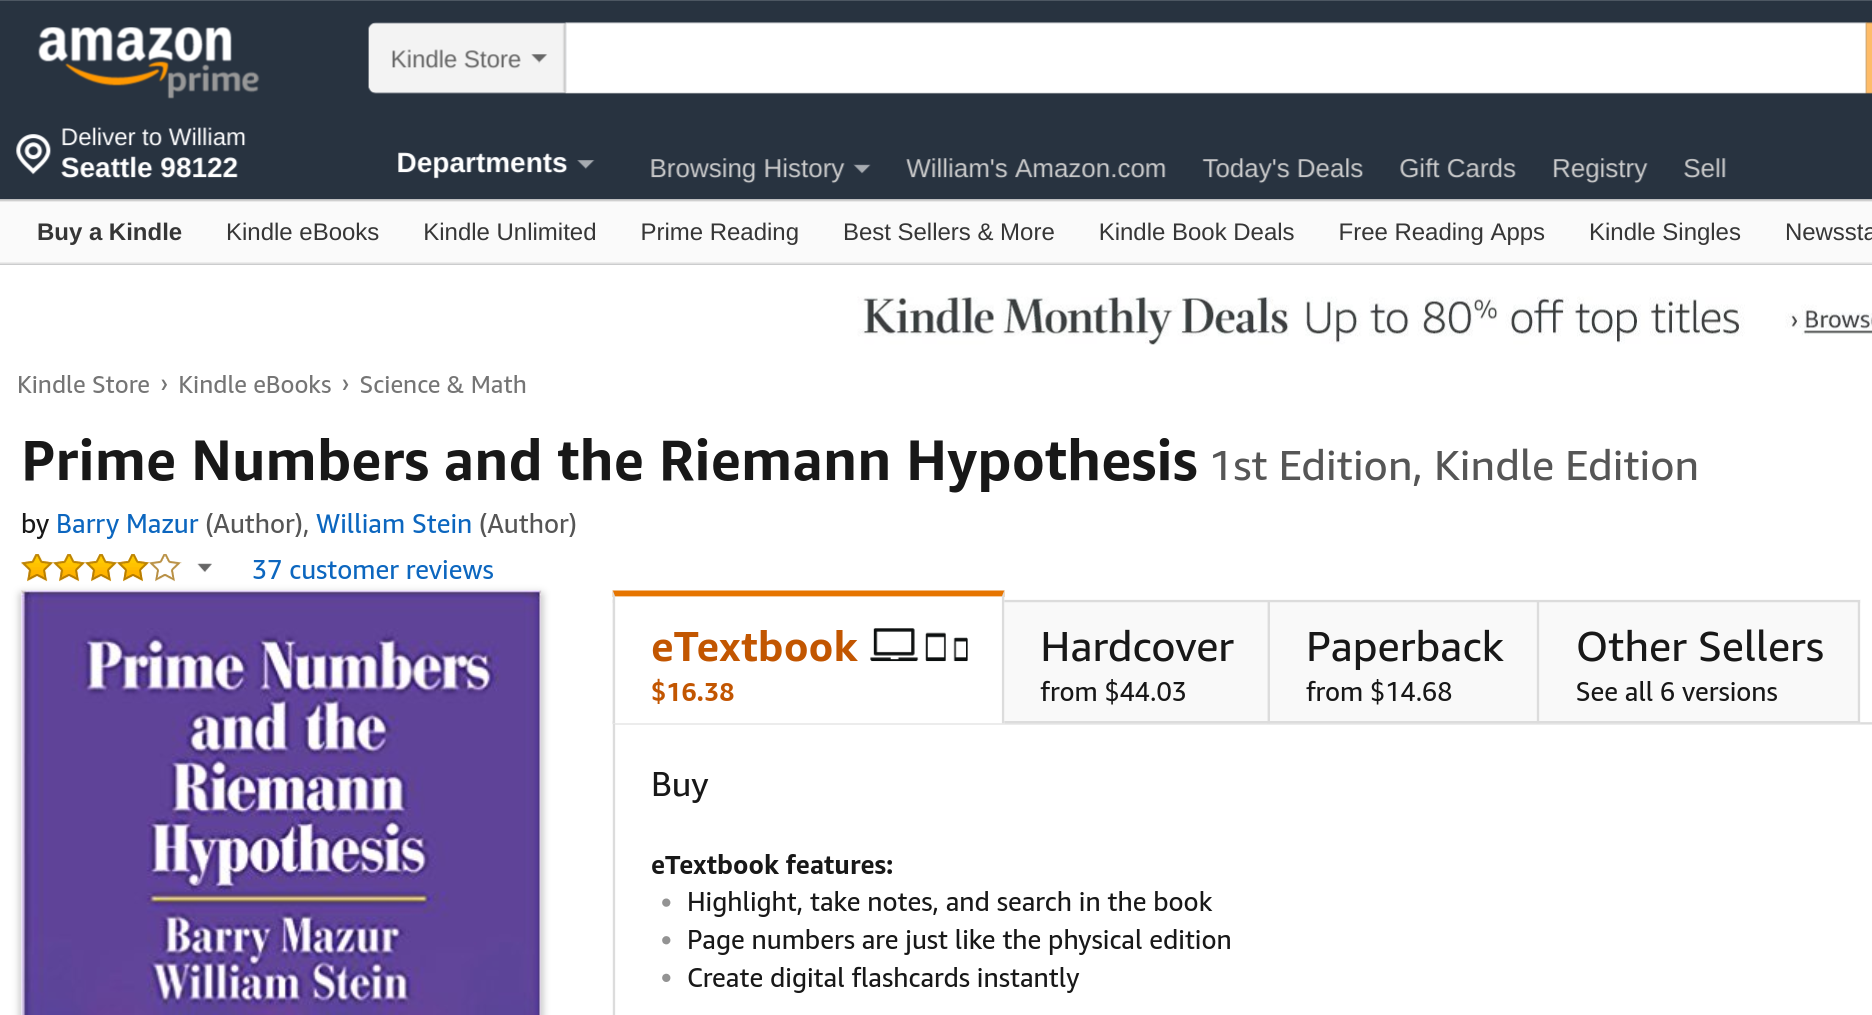
\includegraphics[width=.98\textwidth]{pics/amazon-prime.png}

\end{frame}



\begin{frame}{Reviews by Readers}

  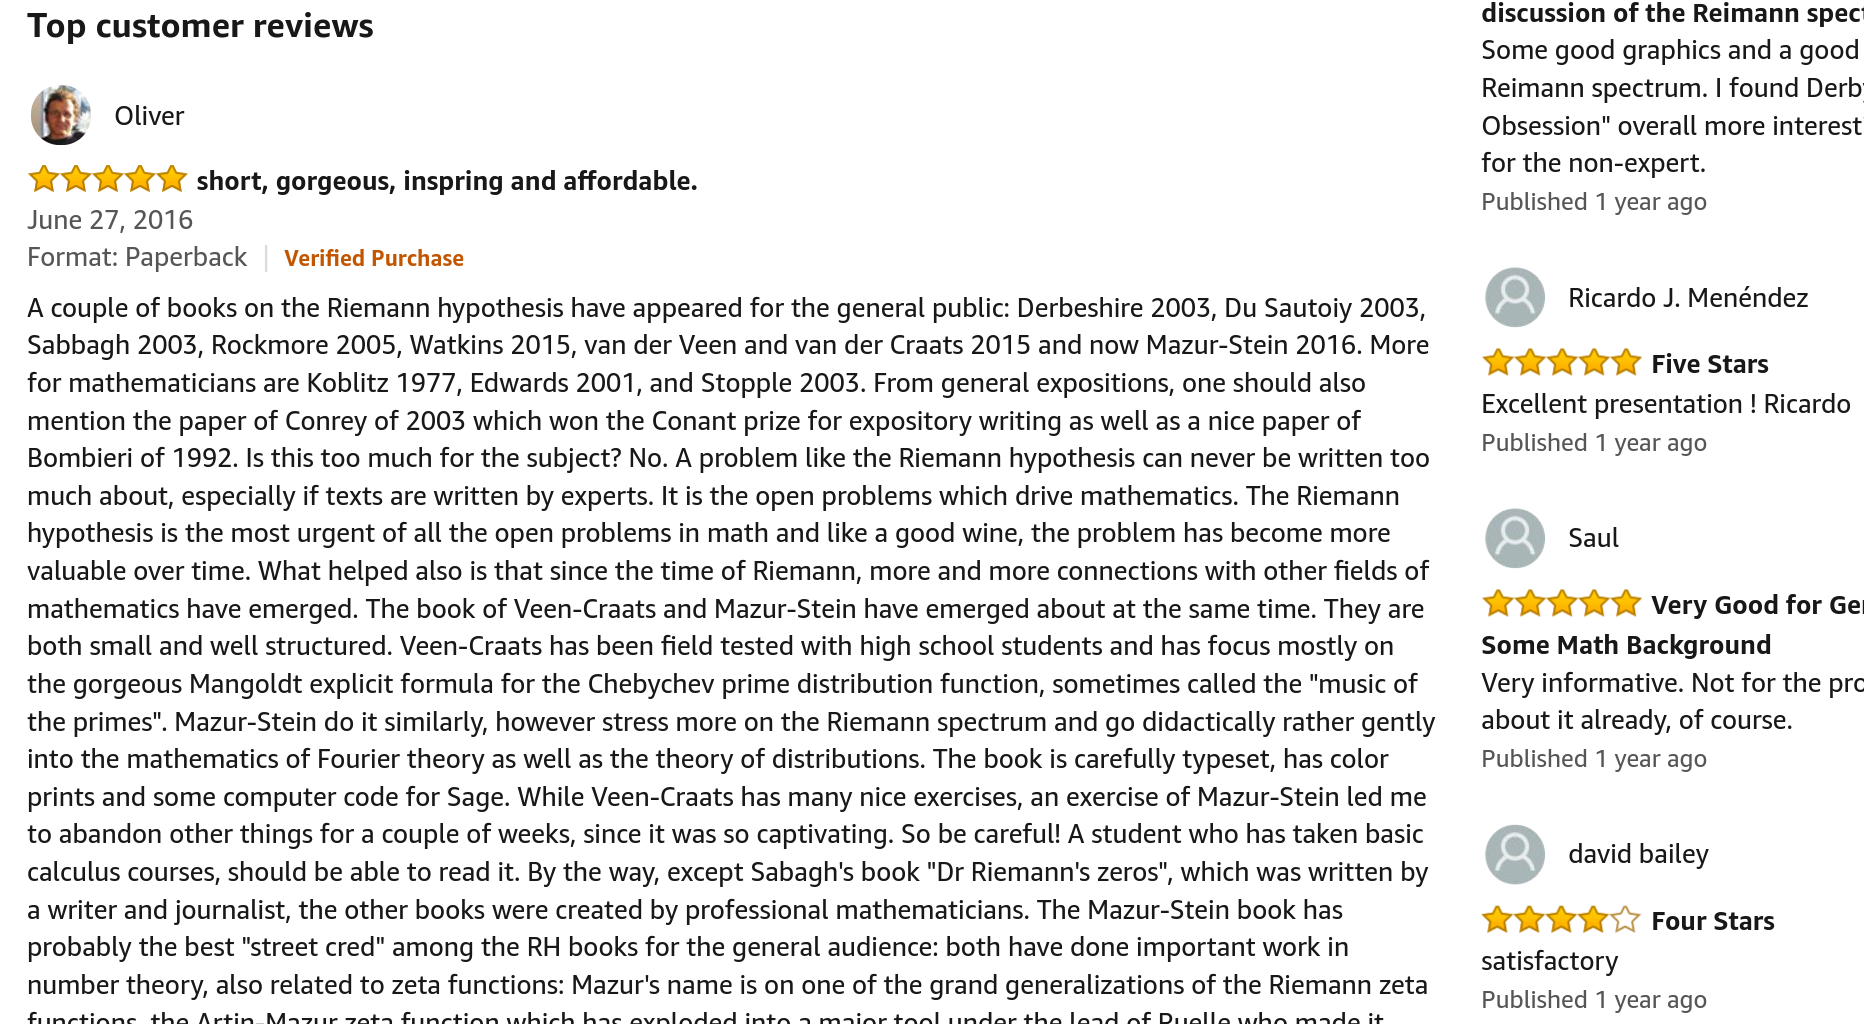
\includegraphics[width=.98\textwidth]{pics/amazon-review.png}

  \vfill

  The negative reviews were due to \textit{production issues}, both with the physical book
  and the Kindle edition....

\end{frame}

\begin{frame}{Reception by Readers}
  \begin{itemize}
    \item Feedback
    \item summarize reviews on amazon
    \item sarnak review in bulletins
    \item other reviews
    \item prizes
  \end{itemize}
\end{frame}

\begin{frame}{Royalties}

  We sold a few copies, so Cambridge University Press sent us checks.
  I bought a puppy (Bella!):

  \begin{center}
    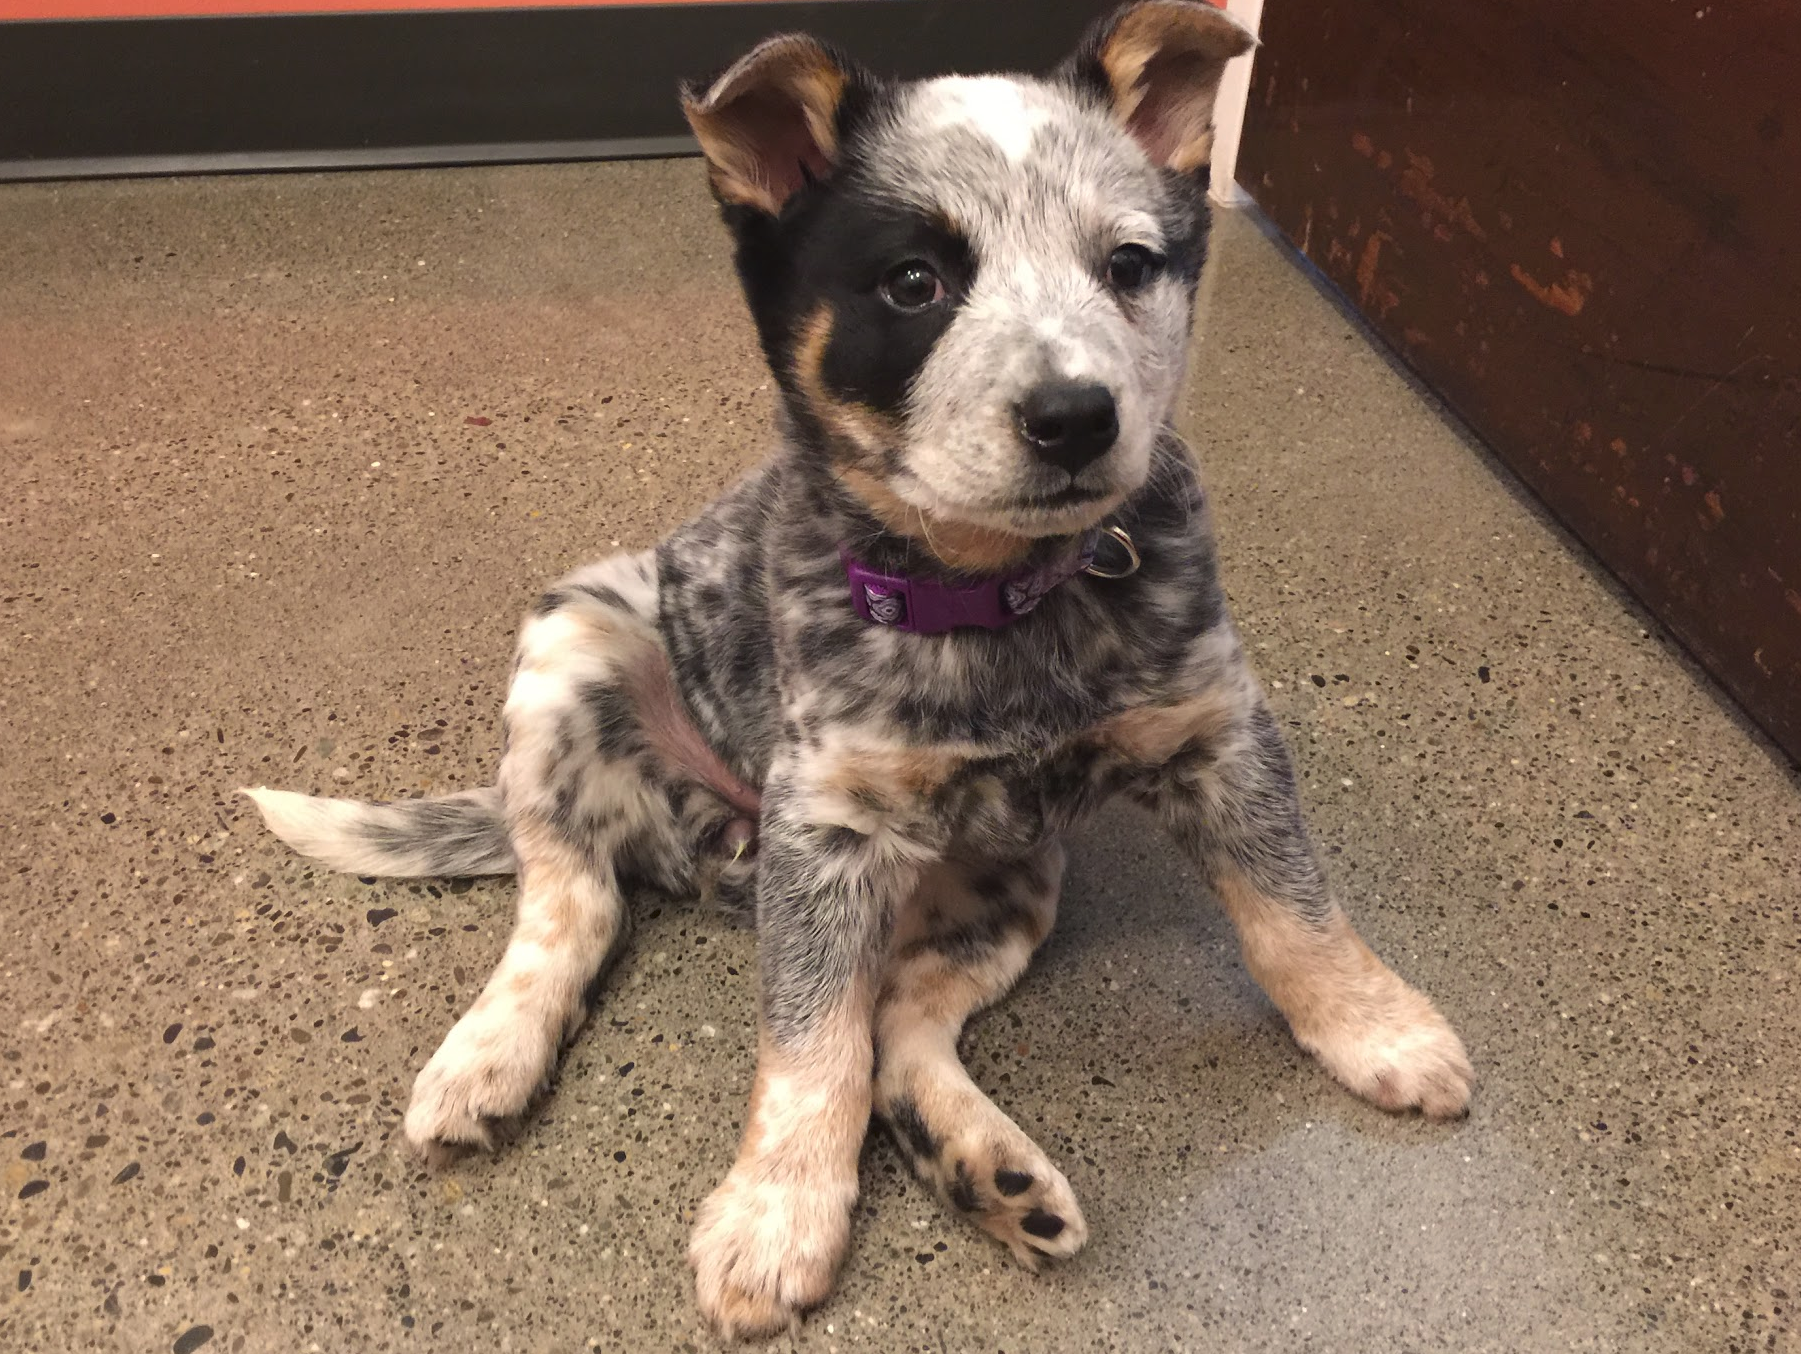
\includegraphics[width=.8\textwidth]{pics/bella-puppy.png}
  \end{center}


\end{frame}


\begin{frame}[fragile]
  \frametitle{Translation: what to expect?}
  \begin{verbatim}
Dear Professor Stein,

Prime Numbers and the Riemann Hypothesis

I am delighted to inform you that we are currently
concluding an agreement with Nippon Hyoron Sha for
a Japanese language edition of your book. They plan
to print an edition of 2,500 copies initially, which
will be sold at approximately 2,200 JPY per copy.

Here is an overview of the terms we have negotiated
...
\end{verbatim}

What to expect?
  \begin{itemize}
    \item  Also Korean?
    \item  Would they bother with French, etc.?  Europeans are very good at English these days.
  \end{itemize}
\end{frame}


\begin{frame}
  \frametitle{Future Plans}
  \begin{itemize}
    \item Online fully interactive version?
    \item Related research on $L$-series of elliptic curves, etc.
  \end{itemize}
\end{frame}


\end{document}